\begin{frame}[c]\label{b.3}
\frametitle{A Theory of Localized Excitations: Numerical Results} % $J_\sigma$

\begin{columns}

\begin{column}{0.6\linewidth}

\onslide<2->\begin{table}[h]
\begin{tabular}{lccccc}
\hline\hline
Glass Former  & Measured$^\ddagger$ $J_\sigma$  & Predicted$^\dagger$ $J_\sigma$  \\ \hline
Poly-(12,0), ($\varepsilon=0.2$)  & \tikzmark{start1} 1.710(2)  & 1.77(2) \tikzmark{end2}  \\
Poly-(12,6), ($\varepsilon=0.2$)    & 0.914(2)  & 0.80(2)   \\
Poly-(18,0), ($\varepsilon=0.0$)    &  6.69(1)  & 10.2(6)   \\
Poly-(18,0), ($\varepsilon=0.2$)    & 2.034(3)  & 2.18(1)   \\
Poly-(10,6), ($\varepsilon=0.1$)    & 1.365(2)  & 1.56(3)  \\
Poly-(10,6), ($\varepsilon=0.2$)    & 0.700(2)  & 0.588(2)   \\
\hline\hline
\only<3->{\begin{tikzpicture}[overlay,remember picture]
  \draw[red, thick] ([shift={(-1ex,1.75ex)}]pic cs:start1) rectangle ([shift={(1ex,-0.75ex)}]pic cs:end2);
\end{tikzpicture}
}
\end{tabular}
\vspace{-12pt}
\caption{\footnotesize $^\ddagger$ Obtained from the rate of particle hopping events in MD simulations.$^\dagger$ Using the final formula, with shear modulus $G^\mathrm{IS}$ and RDF $g(\tilde{r})$ as input. (Hasyim and Mandadapu, \textit{J. Chem. Phys.}, 2021)} \label{tab:summary}
\end{table}
\vspace{-12pt}
\begin{itemize}
    \item<3-> Without fitting to relaxation data, predicted activation energy is in reasonable agreement with MD simulations!
    \item<5-> Strain profile also matches qualitatively with those observed in literature.
\end{itemize}
\end{column}

\begin{column}{0.4\linewidth}

\begin{figure}
    \centering
    \begin{overprint}
    \onslide<4>\centering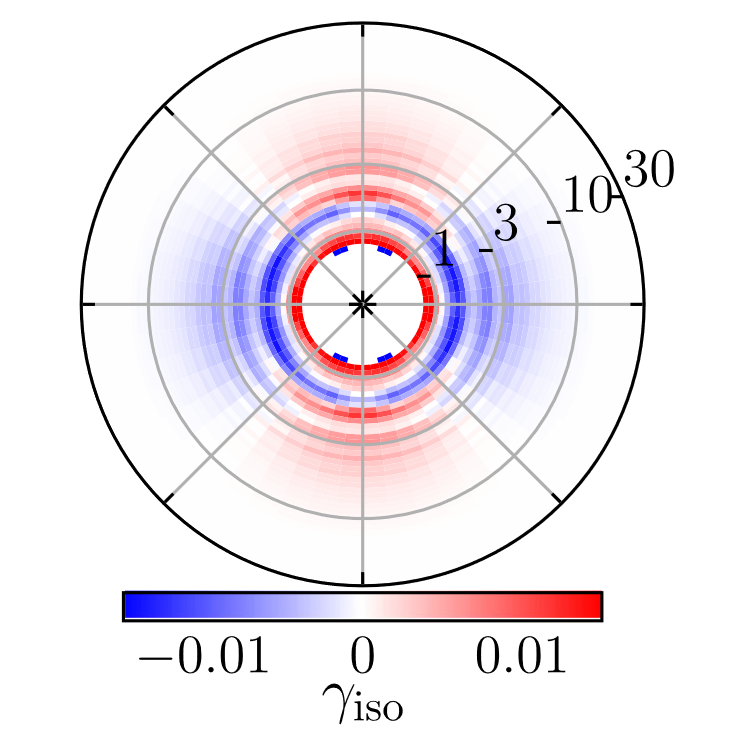
\includegraphics[width=0.95\linewidth]{b.3-exc_results_2/giso_lit.png}\caption{Strain profile from MD simulations (Chacko, et. al. \textit{Phys. Rev. Lett.} 2021)}
    \onslide<5->\centering\includegraphics[width=\linewidth]{b.3-exc_results_2/giso-2.pdf}\caption{From linear theory of elasticity}
    \end{overprint}
    \label{fig:my_label}
\end{figure}

\end{column}

\end{columns}

\end{frame} 